%!TeX root=../thesis.tex

\chapter{Analisis Permasalahan dan Solusi}

  % Pada bab ini akan dipaparkan analisis berdasarkan studi literatur pada bab sebelumnya terkait pembangunan sistem pencegahan intrusi berbasis GPU. Selain itu, akan dipaparkan juga solusi yang diajukan untuk mesin yang akan dibuat.

  \section{Analisis Permasalahan}
  
    % Sistem pencegah intrusi jaringan (NIPS) adalah sistem yang bertugas melakukan penyaringan paket yang dianggap berbahaya. NIPS bekerja dengan cara menangkap paket yang berjalan dalam jaringan untuk kemudian dianalisis. Hasil analisis kemudian ditindaklanjuti berdasarkan \emph{rule} yang telah didefinisikan. Paket dapat ditolak, dibatasi atau bahkan diblok.

    % Analisis paket dapat dilakukan dengan bermacam-macam metode asd

    Dampak dari pengecekan paket adalah adanya \emph{overhead} waktu respons. Lama \emph{overhead} tergantung dari waktu pencocokan pola. Pada sistem pencegah intrusi jaringan (NIPS), hal ini dapat membuat hasil analisis menjadi tidak akurat. Maka perlu adanya metode untuk mempercepat proses analisis. Sebagai perbandingan, \emph{bandwidth} jaringan US Naval Postgraduate School sudah mencapai 20 Gbps dengan traffic rata-rata sebesar 200 Mbps per hari. Sedangkan maksimum paket yang dapat dianalisis secara serial oleh Snort tidak lebih besar dari 300 Mbps \citep{albin2012}.

    Beberapa penelitian tentang teknik mempercepat NIDS dan NIPS telah dilakukan. Desain paling awal yaitu menggunakan desain konkuren dengan \emph{multithreading} pada CPU \citep{multi2004}. Desain ini mampu meningkatkan penggunaan utilitas \emph{thread} CPU secara drastis. Kemudian desain berbeda yang menggunakan GPU mulai diajukan oleh \cite{gnort2008}. Hasil yang didapat mampu mempercepat sistem hingga 5x dibandingkan CPU dengan harga yang sepadan \citep{smith2009}.

    % Pencocokan dapat dilakukan secara stateful, ataupun tidak. Pencocokan yang berbasis stateful akan lebih susah untuk dicek secara paralel.

    %Meski demikian, masih ada beberapa masalah terjadi dalam desain yang telah diajukan. Pencocokan paket masih menggunakan algoritma yang berbasis backtracking sehingga banyak operasi sinkronisasi yang menghambat laju pencocokan dengan multithread.  Selain itu, opsi pada rule seringkali tidak dapat dicocokkan dengan sekali asd

    Berdasarkan pengukuran yang dilakukan oleh \cite{kargus2012}, didapatkan bahwa sebagian besar beban analisa paket berada pada tahap pencarian string pada \emph{payload} paket. Pada tahapan ini, sebagian besar paket yang tidak terindikasi sebagai serangan akan diloloskan. Sehingga beban pencocokan pada tahap berikutnya, yaitu pencocokan \emph{option rule} akan berkurang drastis. Maka, fokus dari solusi yang akan diajukan yaitu implementasi desain yang akan mempercepat kinerja pencocokan string paket pada NIDS Snort.

  \section{Analisis Solusi}

    Eksperimen penggunaan GPGPU pada NIDS akan memodifikasi NIDPS Snort. Snort digunakan karena kode bersifat \emph{open-source} dan mudah untuk dikembangkan, sehingga pengembangan dan eksperimen tidak memerlukan banyak biaya dan dapat dieksplorasi secara mandiri. 

    Pengembangan akan menggunakan platform GPGPU CUDA. Platform CUDA merupakan platform GPGPU yang dibuat pada GPU NVIDIA. Platform CUDA digunakan karena saat ini platform CUDA lebih matang daripada OpenCL. Selain itu, dokumentasi dan contoh CUDA lebih banyak dan API yang lebih sederhana dan spesifik dibanding OpenCL.

    \subsection{Struktur IDS Snort}

      Komponen utama yang akan dioptimasi yaitu pencocokan string yang dilakukan setelah preproses. Pencocokan string dilakukan pada modul MPSE (\emph{multipattern search engine}). Modul ini dipanggil ketika \emph{rule} selesai dikelompokkan berdasarkan servis dan protokol seperti terlihat pada Gambar III.1 di bawah. Tiap \emph{rule group} akan memiliki \emph{instance} MPSE sendiri dan membentuk kamus sesuai \emph{rule} yang ada pada tiap \emph{rule group}.

      \begin{figure}[htb]
        \centering
        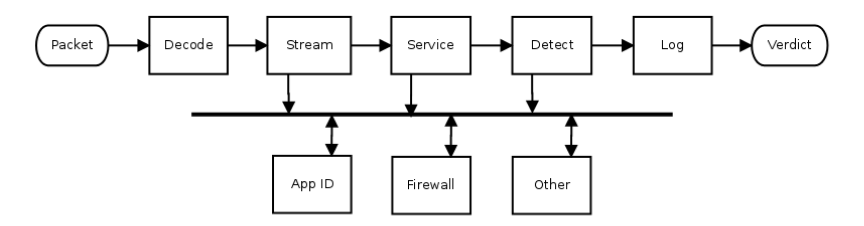
\includegraphics[width=0.8\textwidth]{resources/snort3.png}
        \caption[Arsitektur Snort versi 3]{Arsitektur Snort versi 3. Pencocokan dilakukan pada bagian Detect}
      \end{figure}

      Setelah pembentukan \emph{instance} dilakukan, maka input akan di-\emph{streaming}, dipreproses, dibagi berdasarkan \emph{rule group}, kemudian disuplai ke \emph{instance} MPSE yang terkait. Hasil pencocokan paket akan dikumpulkan dalam \emph{reducer} untuk kemudian dibandingkan dengan \emph{policy} apakah dianggap paket berbahaya atau tidak.

    \subsection{Algoritma Pencocokan \emph{Signature}}

      Komponen utama yang akan dioptimasi yaitu pencocokan string. Diantara pencocokan pola yang digunakan pada Snort, versi Aho-Corasick memiliki runtime yang paling cepat menggunakan teknik \emph{multithreading} pada CPU. Idealnya, modul yang ingin dikembangkan akan melampaui kinerja dari Snort yang menggunakan algoritma Aho-Corasick ini.
      
      Berdasarkan pengujian eksperimen yang dilakukan oleh \cite{lin2013}, implementasi langsung dari algoritma ini tidak memiliki keunggulan yang signifikan pada GPU. Salah satu kendala dari algoritma AC (Aho-Corasick) adalah \emph{boundary matching problem}. Masalah ini bisa diatasi dengan menambahkan jangkauan pencarian sebesar pola terpanjang. Namun, efek dari trik ini adalah peningkatan kompleksitas yang cukup drastis dari $O(n)$ menjadi $O(n + ms)$. 
      
      Solusi yang diajukan oleh \cite{lin2013} yaitu dengan menggunakan algoritma PFAC (\emph{Paralel Failureless Aho-Corasick}). PFAC adalah varian dari AC yang memulai pencocokan \emph{thread} pada tiap karakter dan tidak menggunakan \emph{failure transition}. Ada beberapa keuntungan dari algoritma ini:
    
      \begin{enumerate}

        \item 
        Tiap \emph{thread} hanya bertanggung jawab dengan string yang dimulai dengan karakter pada \emph{thread} tersebut. Ketika tidak ada pola yang cocok dengan huruf pada \emph{thread}, pencarian langsung berhenti pada \emph{thread}. Akibatnya, umur \emph{thread} juga lebih singkat.
        
        \item 
        Dalam mesin PFAC, tiap 32 \emph{thread} dalam \emph{warp} akan mengakses memori yang berurutan dari memori global. Dengan demikian, akses tabel transisi fitur \emph{memory coalescing} dapat dimanfaatkan.
        
        \item
        Tidak memerlukan penyimpanan tambahan untuk \emph{failure transition}. Sehingga konsumsi memori akan lebih sedikit dan kemungkinan \emph{cache hit} lebih besar.
        
      \end{enumerate}
      
      % \subsection{Skema Pengiriman Paket ke GPU}
      
      %  Operasi yang cukup sering akan dilakukan dalam Snort NIPS adalah pengiriman paket dari stream 
      %  Salah satu komponen yang paling penting dalam GPGPU adalah penyalinan data antar host dan device. Pengiriman dari host ke device maupun sebaliknya memiliki \emph{latency} yang cukup besar. Dalam pengujian pada \citep{gnort2008}, didapatkan bahwa \emph{latency} dari transfer payload memiliki runtime lebih dari 80\% runtime total. Sehingga untuk menyembunyikan \emph{latency}, pengujian akan menggunakan batch processing.      
      % pengiriman akan dilakukan per batch. Ukuran batch yang digunakan akan diuji dalam ukuran 32MB, 64MB, 128MB, dan 256MB.
      
      \subsection{Struktur Penyimpanan Kamus}
      
      Implementasi dari mesin PFAC yang digunakan ada beberapa macam. Salah satu model yang dapat digunakan yaitu dengan bentuk seperti pohon dengan \emph{list of pointer} ke status anak. Namun, model yang dialokasi secara dinamis tidak cocok digunakan dalam GPU karena alokasi pada GPU memiliki latensi yang tinggi. Selain itu, lokasi memori dapat menjadi tidak kontigu dan tidak mendukung adanya \emph{spatial locality}.
      
      Opsi lainnya yaitu dengan tabel transisi dua dimensi. Untuk tiap status, akan dibuat daftar status transisi terhadap tiap karakter. Model ini lebih sederhana dan juga mendukung adanya \emph{memory coalescing}. Tabel akan dibentuk di \emph{host memory}. Setelah semua pola didaftarkan, tabel akan disalin ke GPU hanya sebesar ukuran tabel yang terisi agar tidak boros memori. Tiap baris menunjukkan transisi dari tiap status yang bukan status akhir dan memiliki 256 kolom.

      Untuk mengurangi kebutuhan terhadap penanda status akhir, nomor status akan disusun ulang. Status akhir akan diletakkan pada status pertama hingga ke-N. Sedangkan status lainnya termasuk status awal dimulai dari N+1. Dengan demikian, kebutuhan memori untuk penanda akan berkurang. Selain itu, operasi pengecekan dalam kode \emph{kernel} lebih sederhana dan ringan.

      Penghematan memori lebih jauh dapat dilakukan dengan menerapkan skema kompresi tabel menjadi \emph{bitmap}. Namun, keuntungan dari penggunaan memori tekstur akan terhambat. Dibutuhkan komputasi tambahan untuk melakukan \emph{lookup fetch} dari memori tekstur. Sehingga teknik ini tidak digunakan pada rancangan modul.

      \subsection{Alokasi \emph{Thread}}

      Seperti dijelaskan pada bagian III.2.1, \emph{thread} akan menelusuri \emph{state machine} yang sama dan berhenti ketika tidak ada transisi yang valid. Sehingga, banyak diantara \emph{thread} yang akan berhenti sangat awal. Untuk menunjang \emph{stream processor}, \cite{lin2013} mengusulkan alokasi memori yang berulang.

      Dalam satu blok, satu atau beberapa \emph{byte stream} akan ditempatkan sebagai lokasi awal satu \emph{thread}. Misal, dalam blok berisi 4.096 \emph{byte} dengan 512 \emph{thread}, \emph{thread} pertama akan memulai pencocokan pada posisi kelipatan 512. 

      Akibat dari penugasan yang berulang, diharapkan kemungkinan ketimpangan muatan dari masing-masing \emph{thread} akan berkurang. Pengujian yang dilakukan oleh \cite{lin2013} menunjukkan hasil serupa. Sehingga, skema inilah yang akan digunakan dalam implementasi kode \emph{kernel}. %Kode \emph{kernel} akan menerima \emph{stream} sebesar 128 kB dengan 512 \emph{thread}.
      
      % Penyimpanan \emph{signature} mempengaruhi besar memori yang digunakan. Struktur yang digunakan akan menggunakan trie terkompresi. Struktur digunakan untuk memaksimalkan \emph{locality} sehingga mengurangi \emph{latency}. Selain itu, dengan menurunkan konsumsi memori, besar buffer yang dapat digunakan meningkat. Diharapkan, \emph{latency} dari pengiriman juga menurun.
      
      % Penggunaan texture memory diharapkan dapat membantu menurunkan latency dalam pembacaan tabel.
      
      \subsection{Optimasi Latensi pada GPU}
      
      Pencocokan pola dengan tabel transisi adalah aplikasi yang \emph{memory-bound}. Penyimpanan pola pada memori global adalah salah satu sumber latensi. Salah satu optimasi yang dapat digunakan yaitu menyimpan pola pada memori tekstur. Memori tesktur dapat digunakan untuk mengurangi latensi pada simpul yang berdekatan dalam dua dimensi. Berdasarkan \cite{lin2013}, penggunaan memori tekstur dapat menurunkan latensi hingga 12\%. Lebih lanjut, dapat dilakukan pemuatan baris pertama tabel transisi, yaitu baris milik status awal, ke dalam \emph{shared memory} karena baris ini yang pasti akan digunakan semua \emph{thread}. Peningkatan dari memuat baris pertama ke \emph{shared memory} akan berdampak besar ke latensi sistem.
      
      % Memori konstanta unggul ketika pola yang dicocokkan sedikit bercabang. Jika pola yang dicocokkan sedikit bercabang, maka \emph{cache} dapat dimanfaatkan dan latensi berkurang secara signifikan. Namun, pada ruleset Talos, tidak banyak rule yang sama sehingga juga akan banyak terjadi \emph{cache miss}. Akibatnya memori konstanta tidak lagi unggul. 
      
      Kemudian sumber latensi kedua adalah mengambil karakter dari \emph{stream} masukan. Ketika pencocokan dilakukan, \emph{thread} yang bersebelahan akan mengakses karakter dalam \emph{stream input} yang sebelumnya diakses oleh \emph{thread} lain. Berdasarkan skenario ini, \cite{lin2013} mengusulkan untuk menyalin string masukan ke \emph{shared memory} terlebih dahulu. Selain itu untuk mencegah masukan pada memori global terkena \emph{swap}, maka \emph{stream buffer} akan menggunakan \emph{pinned memory}. 

  \section{Rancangan Solusi}

    Pembahasan mengenai rancangan solusi dibagi menjadi 3 bagian. Bagian pertama dibahas mengenai gambaran umum solusi. Bagian kedua dibahas mengenai kebutuhan perangkat lunak. Bagian ketiga dibahas arsitektur perangkat lunak. 

    \subsection{Gambaran Umum Solusi}

      Berdasarkan  analisis  yang  telah  dilakukan, terpilih beberapa metode yang akan digunakan dalam NIDS yang akan dibangun. Metode pengembangan akan mengacu pada eksperimen \cite{lin2013} dengan sedikit penyesuaian untuk \emph{buffer payload} yang mengacu pada \cite{gnort2008}.
      
      % Algoritma pencocokan yang akan digunakan adalah PFAC. Tabel transisi akan menggunakan tabel dua dimensi dengan jumlah kolom sebesar ukuran karakter, yaitu 256 \emph{byte}. Kemudian tabel ini akan diikat ke memori tekstur. Sedangkan \emph{buffer payload} akan menggunakan metode \emph{batching} dengan \emph{pinned memory}.

      Secara garis besar, terdapat 4 tahapan yang harus dilakukan dalam modul pencocokan pola yang akan dibangun:

      \begin{enumerate}

      \item
      Pembentukan tabel transisi \\
      Pembentukan tabel transisi akan dilakukan saat persiapan pencocokan. Pembentukan dilakukan pada \emph{host} kemudian baru akan ditransfer ke \emph{device}. Pembentukan tabel transisi dilakukan dengan mengumpulkan pola terlebih dahulu. Setelah pola terkumpul, lalu simpul akan disusun kembali agar simpul akhir berada di bagian paling awal tabel. 

      \item
      Persiapan tabel transisi dalam \emph{device memory} \\
      Setelah tabel transisi dibentuk, tabel akan dikirimkan ke \emph{device memory}. Penyimpanan pola akan diikat pada memori tekstur. Selain itu juga disiapkan tabel untuk menampung hasil pencocokan. Tabel akan dialokasikan sebesar jumlah \emph{thread} yang digunakan dalam pencocokan.

      \item
      Penelusuran automata \\
      Pencocokan dilakukan dengan penelusuran mesin PFAC yang sudah dibentuk. String masukan akan dimuat pada \emph{shared memory}. Tiap \emph{thread} akan memulai pencocokan pada satu karakter di string masukan. Penelusuran dilakukan hingga mencapai status akhir. Jika status akhir bukan merupakan status dummy, maka hasil pencocokan akan diset pada tabel yang berada di global memori.

      \end{enumerate}

    \subsection{Kebutuhan Perangkat Lunak}

      Berdasarkan analisis yang dilakukan sebelumnya, NIDS yang akan dibangun setidaknya memiliki spesifikasi kebutuhan fungsional seperti yang dijabarkan dalam Tabel III.1.
      
      \begin {table}[h]
\begin{center}
\caption {Kebutuhan Fungsional}
\begin{tabular}{|p{.5cm}|l|}

\hline
\rowcolor{gray!10}
No & Kebutuhan Fungsional \\
\hline

1 & Mampu membaca paket dari berkas PCAP \\
\hline

2 & Mampu membuat struktur automata untuk pencocokan paket \\
\hline

3 & Mampu menjalankan pencocokan pada GPU \\
\hline

4 & Mampu menghasilkan \emph{alert} pada paket yang terindikasi berbahaya \\
\hline

\end{tabular}
\end{center}
\end{table}


      % Berdasarkan Kebutuhan fungsional tersebut maka diagram \emph{use case} dari NIDS yang akan dibangun adalah seperti pada Gambar III.1 berikut

      % \begin{figure}[htb]
  \centering
  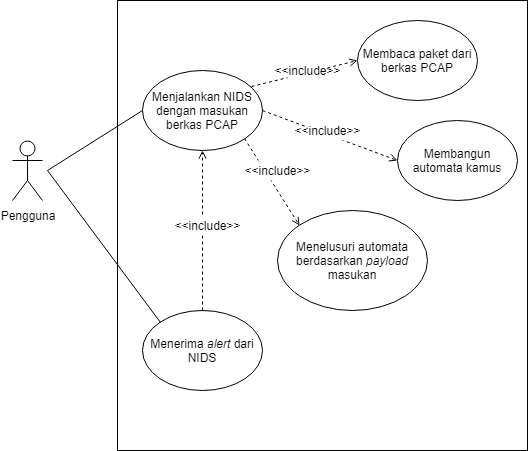
\includegraphics[width=1.0\textwidth]{resources/use-case.png}
  \caption[Diagram \emph{Use Case}]{Diagram \emph{Use Case}}
\end{figure}

    \subsection{Arsitektur Perangkat Lunak}

      Arsitektur yang digunakan akan menggunakan arsitektur dasar Snort. Dalam mengimplementasikan modul pencocokan, Snort menyediakan API yang dapat diimplementasi dengan mudah. Sehingga dalam penggabungan modul tersebut, hanya perlu dibuat \emph{wrapper} untuk memanggil modul yang telah diimplementasi secara terpisah.

      Modul akan terdiri dari beberapa komponen. Komponen-komponen tersebut akan tersusun menjadi sebuah \emph{pipeline} seperti pada Gambar III.1. Ada beberapa komponen utama dalam modul pencocokan pola:

      \begin{figure}[htb]
  \centering
  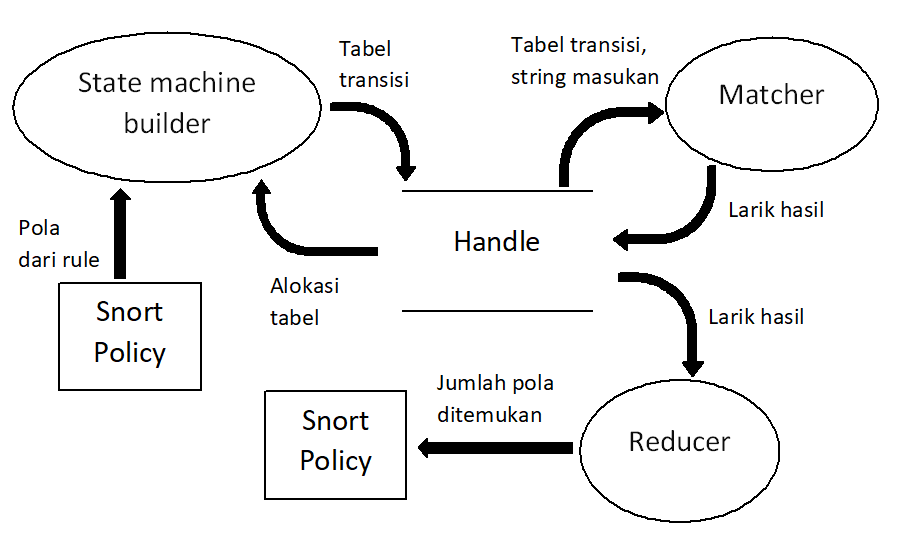
\includegraphics[width=0.5\textwidth]{resources/module-arch.png}
  \caption[Arsitektur modul]{Arsitektur modul}
\end{figure}
      
      \begin{enumerate}

        \item 
        \emph{Pattern builder} \\
        \emph{Pattern builder} melakukan pembangkitan kamus dari \emph{ruleset}. Pola akan ditambahkan dalam bentuk \emph{list of string} untuk kemudian ditampung dalam \emph{buffer}. Kemudian \emph{buffer} akan diiterasi untuk membentuk kamus. Kamus yang dibentuk menggunakan struktur tabel dua dimensi dengan baris sebagai status dan kolom sebagai status transisi. Setiap baris memiliki kolom sebesar 256 \emph{byte}.

        \item
        \emph{Matcher} \\
        \emph{Matcher} akan menyalin \emph{payload} dari \emph{host buffer} ke \emph{device buffer}. Kemudian dari \emph{buffer} akan disalin ke \emph{shared memory}. Lalu \emph{matcher} akan melakukan pencocokan dengan menelusuri kamus secara paralel berdasarkan tiap karakter.

        \item
        \emph{Reducer} \\
        \emph{Reducer} akan menggabungkan hasil pencocokan dari tiap \emph{byte} sehingga diperoleh jumlah total rule yang terdeteksi. Jumlah ini akan dibandingkan dengan \emph{threshold} untuk menentukan apakah \emph{payload} perlu dilakukan pencocokan lebih lanjut atau tidak. \emph{Reducing} akan dilakukan secara sekuensial pada CPU.
        
      \end{enumerate}